\documentclass[xcolor=pdftex,dvipsnames,table,mathserif,aspectratio=169]{beamer}
\usetheme{metropolis}

%\usetheme{Darmstadt}
%\usepackage{times}
%\usefonttheme{structurebold}

\usepackage[english]{babel}
%\usepackage[table]{xcolor}
\usepackage{pgf,pgfarrows,pgfnodes,pgfautomata,pgfheaps}
\usepackage{amsmath,amssymb,setspace,centernot}
\usepackage[latin1]{inputenc}
\usepackage[T1]{fontenc}
\usepackage{relsize}
\usepackage{stmaryrd}
\usepackage{pdfpages}
\usepackage{booktabs}
\usepackage[absolute,overlay]{textpos} 


\newenvironment{reference}[2]{% 
  \begin{textblock*}{\textwidth}(#1,#2) 
      \footnotesize\it\bgroup\color{red!50!black}}{\egroup\end{textblock*}} 

\DeclareMathSizes{10}{10}{6}{6} 
\AtBeginSection[]{
  \begin{frame}
  \vfill
  \centering
  \begin{beamercolorbox}[sep=8pt,center,shadow=true,rounded=true]{title}
    \usebeamerfont{title}\insertsectionhead\par%
  \end{beamercolorbox}
  \vfill
  \end{frame}
}
\begin{document}
\title{Diversion Ratios}
\author{Chris Conlon}
\institute{Grad IO}
\date{\today}

\frame{\titlepage}
\section{What are Diversion Ratios?} 

\begin{frame}{Horizontal Merger Guidelines (2010 rev.)}
\begin{quote}
In some cases, the Agencies may seek to quantify the extent of direct competition between a product sold by one merging firm and a second product sold by the other merging firm by estimating the diversion ratio from the first product to the second product. The diversion ratio is the \alert{fraction of unit sales lost by the first product due to an increase in its price that would be diverted to the second product}. Diversion ratios between products sold by one merging firm and products sold by the other merging firm can be very informative for assessing unilateral price effects, with \alert{higher diversion ratios indicating a greater likelihood of such effects}. Diversion ratios between products sold by merging firms and those sold by \alert{non-merging firms have at most secondary predictive value.}
\end{quote}
\end{frame}

\begin{frame}{This time with equations}
 Raise price of good $j$. People leave. What fraction of leavers switch to $k$?
\begin{eqnarray*}
D_{jk} (p_j,p_{-j})= \frac{\frac{\partial q_k}{\partial p_j}}{\left|\frac{\partial q_j}{\partial p_j} \right|}
\end{eqnarray*}
It's one of the best ways economists have to characterize competition among sellers.
\begin{itemize}
\item High Diversion: Close Substitutes $\rightarrow$ Mergers more likely to increase prices.
\item Very low diversion $\rightarrow$ products may not be in the same market.\\ (ie: Katz \& Shapiro). This is just hypothetical monopolist or SSNIP test.
\item Demand Derivatives NOT elasticities.
\item No equilibrium responses.
\end{itemize}
\end{frame}

\begin{frame}
\frametitle{Unilateral Effects}
\begin{itemize}
\item Eliminating competition between the merging firms can itself constitute a substantial lessening of competition
\item Developed in the 1992 Guidelines, and larger role in the 2010 Guidelines
\item Based on modern theoretical literature: Farrell Shaprio (1990), Werden (1996), Farrel Shapiro (2010), Froeb and Werden (1998)
\item Extension to multiple products/firms may be tricky (Carlton 2010, Hausman, Moresei, Rainey (2010)).
\item Doesn't go as far as pass-through literature (Bulow Geanakoplos Klemperer (1985), Jaffe Weyl (2013)). 
\item Limited empirical results in academic literature: (Cheung 2013, Miller, Remer, Ryan, Sheu (2013), Conlon Mortimer (2013/2015/2020...))
\item Possibly more empirical experience at DOJ/FTC.
\end{itemize} 
\end{frame}


%\begin{frame}
%\frametitle{Antitrust Policy -- Horizontal Mergers}
%Antitrust authorities use diversion ratios, a la Bertrand, to understand the `unilateral effects' of proposed mergers.
%\begin{itemize}
%\item Unilateral effects: competition between products of the merged firm is reduced because the merged firm internalizes substitution between jointly-owned products.
%\item Unilateral effects can lead to price increases.
%\item Current U.S. merger guidelines:\\
%\indent \textit{\footnotesize Diversion ratios between products [of the merging firms] can be very informative for assessing unilateral price effects.}
%\item Higher diversion between merging products pre-merger $\rightarrow$ greater scope for potential price increases.
%\end{itemize}
%\end{frame}

\section{Where do Diversion Ratios come from?\\ (Stolen from Conlon and Mortimer (2020)}
\begin{frame}{In Theory}
\footnotesize
Consider Bertrand FOC's for single-product firm $j$, buys $k$:
\begin{align*}
\arg \max_{p_j}&\, (p_j-c_j) \cdot q_j(p_j,p_{-j}) + (p_k-c_k) \cdot q_k(p_j,p_{-j})\\
0 &=q_j+ (p_j-c_j) \cdot \frac{\partial q_j}{\partial p_j}+ (p_k-c_k) \cdot  \frac{\partial q_k}{\partial p_j}\\
p_j &=-q_j/\frac{\partial q_j}{\partial p_j}+ c_j + (p_k-c_k) \cdot  \underbrace{\frac{\partial q_k}{\partial p_j}/-\frac{\partial q_j}{\partial p_j}}_{D_{jk}}\\ \pause
p_j &= \underbrace{\frac{\epsilon_{jj}}{\epsilon_{jj}+1}}_{\text{Lerner Markup}} \left[  c_j -\overbrace{ \underbrace{c_j \cdot e_j}_{\text{efficiency}} + \underbrace{(p_k-c_k) \cdot  D_{jk} (p_j,p_{-j})}_{\text{opp cost}}}^{UPP} \right]\\
\end{align*}
Caveat: UPP, Partial Merger, Full Merger.
\end{frame}


\begin{frame}
\frametitle{UPP Extensions}
\begin{block}{Extension to multiple acquisitions:}
Very easy if we have that $p_j - mc_j = p - mc$ are the same for several values of $j$.  Then
\begin{eqnarray*}
UPP_j &\approx& (p - mc) \sum_k D_{jk}(\mathbf{p}) -  E_j mc_j \\
\end{eqnarray*}
\end{block}
If several brands of acquisition have the same markup -- can consider firm-level diversion. (We can aggregate diversion across similar flavors)
\begin{block}{Ignoring Efficiencies}
\begin{eqnarray*}
GUPPI_j &\approx& \frac{(p_j - mc_j)}{p_j} D_{jk}(\mathbf{p}) \\
\end{eqnarray*}
\end{block}

\end{frame}



\begin{frame}
\frametitle{Diversion: In Practice}
\footnotesize
\begin{enumerate}
\item Calculated from an estimated demand system (ratio of estimated cross-price to own-price demand derivatives)
\item Consumer surveys (what would you buy if not this?)
\item Obtained in `course of business' (sales reps, internal reviews)
\end{enumerate}
Antitrust authorities may prefer different measures in different settings. Are they concerned about:
\begin{itemize}
\item Small but widespread price hikes?
\item Product discontinuations or changes to availability?
\end{itemize}
Is it sufficient to rely on data from merging firms only?
\begin{itemize}
\item Do we need diversion to other products in the `market' or other functions of market-level data?
\item Discrete-choice demand models imply that `aggregate diversion' (including to an outside good) sums to one.
\end{itemize}
\end{frame}



\section*{A Simple Insight...}

\begin{frame}
\frametitle{Diversion has treatment effects interpretation}
\begin{description}[labelwidth=\widthof{\bfseries Treated group}]
\item[Treatment] ``not purchasing $j$"
\item[Outcome] fraction of $j$ consumers who switch to product $k$
\item[Treated group] consumers who would have purchased $j$ at pre-merger price, but do not purchase at a higher price
\end{description}

Heterogeneity: Individuals who leave $j$ after a \$0.01 price increase differ in their taste for $k$ from those who leave after \$1, \$100, \$10,000 price increases.
\end{frame}


%\begin{frame}
%\frametitle{Experimental Interpretation}
%  \setbeamertemplate{description item}[align left]
%\begin{description}
%\item[Population:] All individuals who, at current prices $(p_j^0,p_{-j})$, buy $j$.
%\item[Treatment Group:] Individuals who buy $j$ at $(p_j^0,p_{-j})$, but would not buy at $(p_j^0+\Delta p_j,p_{-j})$ -- denoted $\Delta q_j$.
%\item[Outcome:] Fraction of treatment group who purchase $k$ instead.
%\item[Population of Interest:] Individuals purchasing $j$ who are most price-sensitive -- i.e., those who would leave $j$ after an infinitesimal price increase. 
%In another context, we may care about all individuals who buy $j$ at $(p_j^0,p_{-j})$.
%\item[Instrument:] $\Delta p_j$ functions as the instrument -- it monotonically increases probability of treatment. 
%\end{description}
%\end{frame}

\begin{frame}{Start with the Wald Estimator}
Consider an experiment designed to measure diversion, where everything else is held fixed and $p_j$ is exogenously increased by $\Delta p_j$:
\begin{eqnarray*}
\small
D_{jk}(p_j,p_{-j}) &=&  \left| \frac{q_{k}(p_j+\Delta p_j,p_{-j}) - q_{k}(p_j,p_{-j})}{q_{j}(p_j+\Delta p_j,p_{-j}) - q_{j}(p_j,p_{-j})}   \right|  \\
&=& 
 \frac{\int_{p_j^{0}}^{p_j^0+\Delta p_j}  \frac{\partial q_k(p_j,p_{-j})}{\partial p_j}\,\partial p_j }{\Delta q_j}
\end{eqnarray*}
\end{frame}

\begin{frame}{Re-write as Local Average Treatment Effect}
\begin{eqnarray*}
\widehat{D_{jk} }^{LATE}&=& \frac{1}{\Delta q_j} \int_{p_j^{0}}^{p_j^{0}+\Delta p_j} D_{jk}(p_j,p_{-j}) \left| \frac{\partial q_j (p_j,p_{-j})}{\partial p_j} \right|\, \partial p_j
\end{eqnarray*}
\begin{itemize}
\item $\widehat{D_{jk}}^{LATE}$ is a Local Average Treatment Effect \alert{(LATE)}.
\begin{itemize}
\item Identified from finite price changes (simulated or actual).
\item For any finite price increase, we measure a weighted average of the diversion function, where the weights are the lost sales of $j$:  $w(\mathbf{p}) = \frac{1}{\Delta q_j} \frac{\partial q_j(p_j,p_{-j})}{\partial p_j} $
\end{itemize}
\pause
\item Let $\widehat{D_{jk}}^{ATE}$ denote Average Treatment Effect \alert{(ATE)} when everyone is treated.
 \begin{itemize}
\item $\Delta p_j$ increases to \alert{choke price}:  $Q_j(p_j^0 + \Delta p_j, p_{-j}) = 0$.
\item Interpretation as second-choice data.
\end{itemize}
\end{itemize}
\end{frame}



\begin{frame}{The Nonparametric Object: MTE}
Re-writing:
\begin{eqnarray*}
\widehat{D_{jk}}^{LATE}(p_j,p_{-j})&=& \frac{1}{\Delta q_j} \int_{p_j^{0}}^{p_j^{0}+\Delta p_j} D_{jk}(p_j,p_{-j}) \left| \frac{\partial q_j (p_j,p_{-j})}{\partial p_j} \right|\, \partial p_j
\end{eqnarray*}
\begin{itemize}
\item Diversion, $D_{jk}(p_j,p_{-j})$, is a Marginal Treatment Effect \alert{(MTE)}  in the language of Heckman and Vytlacil (1999).
\item It is a \alert{function}. Actually a \alert{matrix valued function}.
\item It is not identified non-parametrically from a single price increase.
\end{itemize}
\end{frame}

\begin{frame}
\frametitle{Various Treatment Effects}
\begin{itemize}
\item Determine what different measures of diversion identify.
\begin{itemize}
\item Finite price increase $\rightarrow$ local average treatment effect (LATE)
\item Product removal (treating everyone) $\rightarrow$ average treatment effect (ATE)
\item A nonparametric function of $p_j$ $\rightarrow$ marginal treatment effect (MTE) 
\item Constant diversion: three measures coincide (Theory/Empirics)
\end{itemize}
\end{itemize}
 But... How do the weights work? An illustration.
 \end{frame}




%\begin{frame}
%\frametitle{Experimental Interpretation (Conlon and Mortimer 2015)}
%\begin{description}
%\item[Population] All individuals who at current prices would buy $j$.
%\item[Treatment] Not buying $j$.
%\item[Outcome] Fraction who purchase $k$ instead.
%\item[Instrument] $p_j$ functions as the instrument (it monotonically increases probability of treatment).
%\item[Effect of Interest] treat only those individuals purchasing $j$ who are most price-sensitive. (ie: those who would leave  $j$ after a 5-10\% price increase).
%\end{description}
%\end{frame}

%\begin{frame}{Diversion Experiments}
%\begin{itemize}
%\item Consider an experiment designed to measure diversion, where everything else is held fixed and $p_j$ is increased by $\Delta p_j$ 
%\begin{eqnarray*}
%\widehat{D_{jk}} &=& \left| \frac{\Delta Q_{k}}{\Delta Q_j} \right| =  \left| \frac{Q_{k}(\mathbf{p^{(1)}}) - Q_{k}(\mathbf{p^{(0)}})}{Q_{j}(\mathbf{p^{(1)}}) - Q_{j}(\mathbf{p^{(0)}})}   \right| = \frac{\int_{p_j^{0}}^{p_j^1}  \frac{\partial q_k(p_j,p_{-j})}{\partial p_j}\,\partial p_j }{\int_{p_j^{0}}^{p_j^1}   \frac{\partial q_j(p_j,p_{-j})}{\partial p_j} \, \partial p_j}
%\end{eqnarray*}
%\end{itemize}
%\end{frame}

%\begin{frame}{Diversion: Finite Price Change}
%Think about the \alert{Local Average Treatment Effect}:
%\begin{eqnarray*}
%\widehat{ED_{jk} }&=& \frac{1}{\Delta q_j} \int_{p_j^{0}}^{p_j^{0}+\Delta p_j} \underbrace{\frac{\partial q_k}{\partial q_j}}_{D_{jk}(\mathbf{p})} \left| \frac{\partial q_j}{\partial p_j} \right|\, \partial p_j
%\end{eqnarray*}
%\begin{itemize}
%\item Our estimated diversion measure is a weighted average of diversion, where the weights are the fraction of lost sales of $j$:  $w(\mathbf{p}) = \frac{1}{\Delta q_j} \frac{\partial q_j}{\partial p_j} (\mathbf{p})$
%\item If demand declines quickly near the market price $ATE \approx D_{jk}(\mathbf{p})$ at $\mathbf{p}^{(0)}$.
%\end{itemize}
%\end{frame}

\begin{frame}
\frametitle{Thought Experiment -- Linear Demand for a Toyota Prius}
\begin{center}
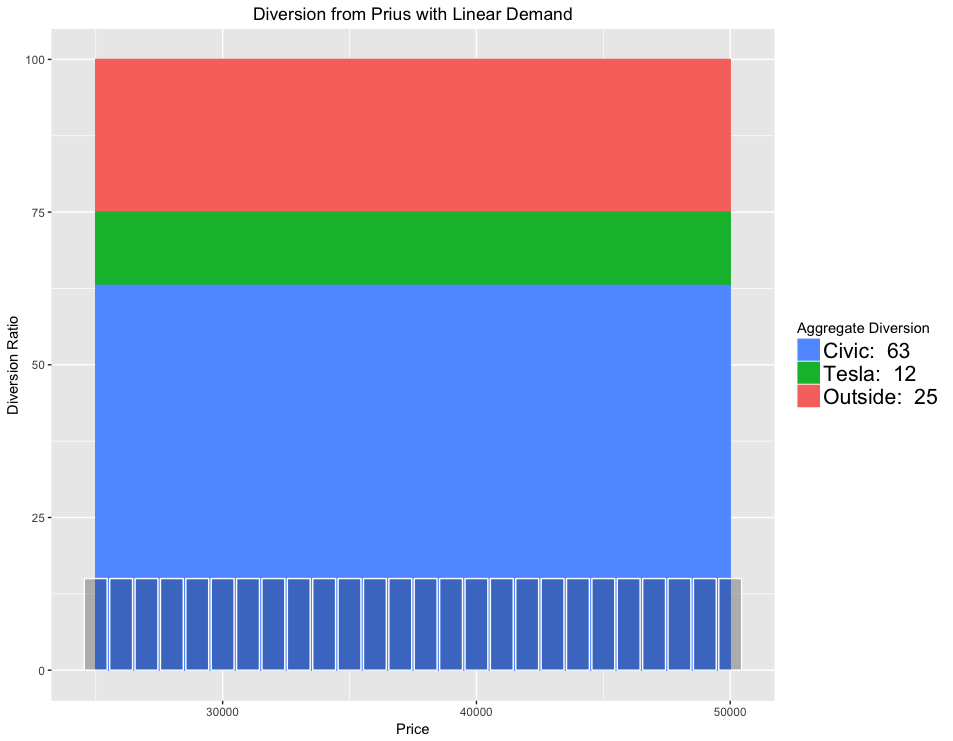
\includegraphics[width=4in]{./resources/new_prius_linear.png}
\end{center}
\end{frame}

\begin{frame}
\frametitle{Thought Experiment -- Inelastic CES Demand for a Prius}
\begin{center}
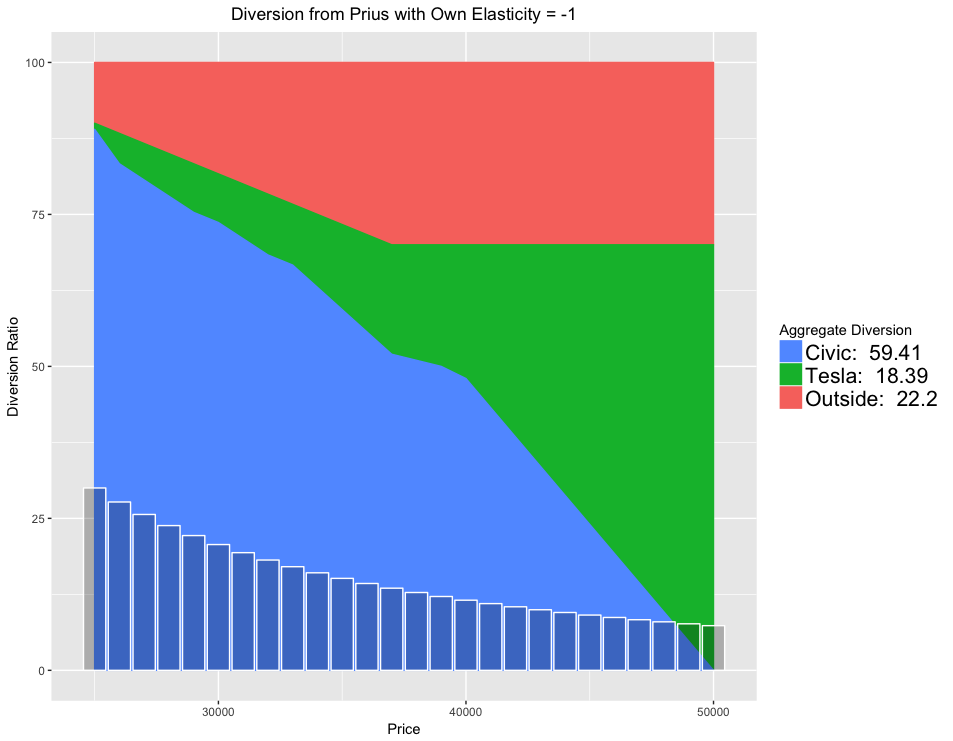
\includegraphics[width=4in]{./resources/new_prius1.png}
\end{center}
\end{frame}

\begin{frame}
\frametitle{Thought Experiment -- Elastic CES Demand for a Prius}
\begin{center}
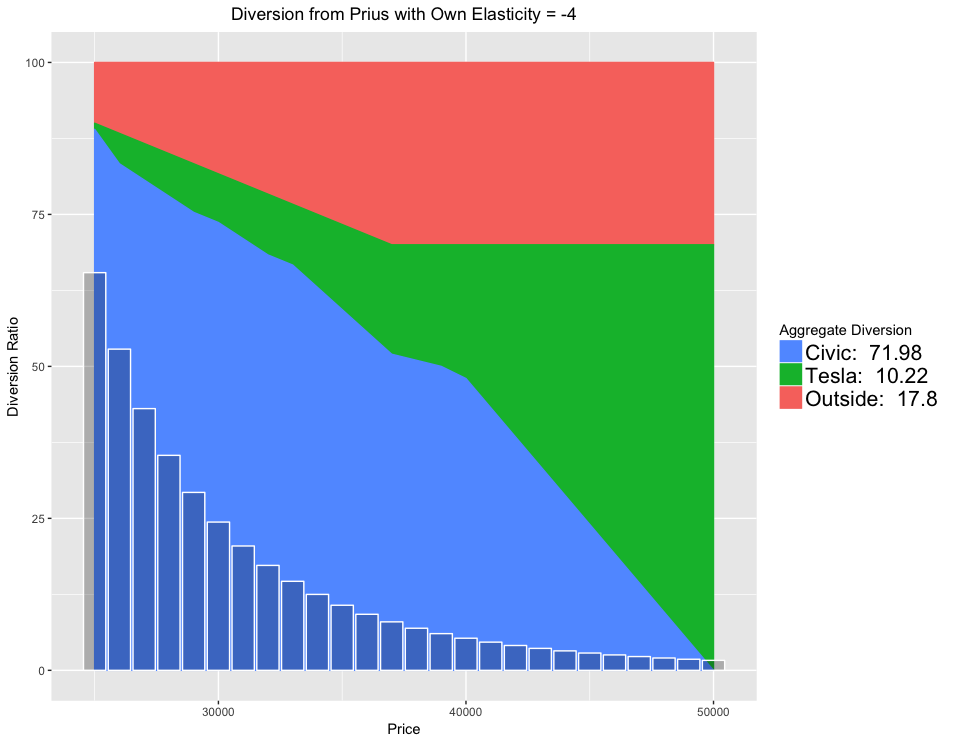
\includegraphics[width=4in]{./resources/new_prius4.png}
\end{center}
\end{frame}


\begin{frame}
\frametitle{Bias of Estimator}
\footnotesize
How far apart are $D_{jk}(\mathbf{p^0})$ and $\widehat{D_{jk}}$ when we increase price by $\Delta p_j$? 
\begin{eqnarray*}
\nonumber q_k(\mathbf{p}+ \Delta p_j) &\approx& q_k(\mathbf{p}) + \frac{\partial q_k}{\partial p_j} \Delta p_j + \frac{\partial^2 q_k}{\partial p_j^2} (\Delta p_j)^2 + O((\Delta p_j)^3) \\
\frac{ q_k(\mathbf{p}+ \Delta p_j)-q_k(\mathbf{p}) }{\Delta p_j} &\approx& \frac{\partial q_k}{\partial p_j}+ \frac{\partial^2 q_k}{\partial p_j^2} \Delta p_j + O(\Delta p_j)^2 \\
Bias(\widehat{D_{jk}} -D_{jk}(\mathbf{p^0})) &\approx& -  \frac{D_{jk} \frac{\partial^2 q_j}{\partial p_j^2} +  \frac{\partial^2 q_k}{\partial p_j^2} }{\frac{\partial q_j}{\partial p_j} + \frac{\partial^2 q_j}{\partial p_j^2}\Delta p_j } \Delta p_j
\end{eqnarray*}
\begin{itemize}
\item The downside of a large change $\Delta p_j$ is that the approximation of demand at $\mathbf{p^0}$ is less accurate and depends on the curvature of the demand function.
\item There are two demand models for which $Bias \equiv 0$ \alert{(constant treatment effects)}: \pause linear demand and plain IIA logit.
\end{itemize}
\end{frame}

\begin{frame}
\frametitle{Variance of Estimator}
\footnotesize
\begin{eqnarray*}
Var(\widehat{D_{jk} })&\approx& Var\left( \frac{\Delta q_k}{|\Delta q_j|} \right)\approx \frac{D_{jk} (1-D_{jk})}{\Delta q_j} \approx \frac{D_{jk} (1-D_{jk})}{\left| \frac{\partial q_j}{\partial p_j} \right| \Delta p_j}
\end{eqnarray*}
\normalsize
Variance is a problem when:
\begin{itemize}
\item  $\left| \frac{\partial q_j}{\partial p_j} \right| $ is small (inelastic demand $\rightarrow$ market power/ when we may be most worried about mergers).
\item $\Delta p_j \approx 0 $ (when price change is small).
\item Exacerbated by variation in $(q_j,q_k)$ unrelated to the exogenous price change (stochastic demand).
\end{itemize}
Bias-Variance tradeoff
\begin{itemize}
\item Precise measure of $\widehat{D_{jk}}^{ATE}$ or $\widehat{D_{jk}}^{LATE}$ for a large $\Delta p_j$ vs.
\item Noisy measure of $D_{jk}(\mathbf{p^0})$
\end{itemize}
\end{frame}


\begin{frame}
\footnotesize
\frametitle{Nevo (2000) and BLP (1999) Applications}
Data from Nevo (2000): $T=94$ markets, $J=24$ brands.
\begin{itemize}
\item RTE cereal (e.g., Kellogg's and General Mills merger)
\begin{eqnarray*}
u_{ijt} = d_{j} + x_{jt} \underbrace{(\overline{\beta} + \Sigma\cdot \nu_i + \Pi\cdot d_{it})}_{\beta_{it}} + \Delta \xi_{jt} + \varepsilon_{ijt}
\end{eqnarray*}

\begin{itemize}
\item[-] Features a large amount of preference heterogeneity, especially with respect to the price sensitivity $\beta_{it}^{price}$
\item[-] Estimated coefficient on price is distributed:
\begin{eqnarray*}
\scriptsize
\beta_{it}^{price} \sim N\left(\text{-63 + 588} \cdot \text{income}_{it} \text{ - 30} \cdot \text{inc}^2_{it}  \text{ + 11}\cdot \text{I[child]}_{it}, \sigma \text{=3.3}\right)
\end{eqnarray*}
\end{itemize}
\end{itemize}
%Because we have estimated a fully specified structural demand system, we can calculate the treatment effect measures easily:

Data from BLP (1999): $T=21$ markets, $J \approx 150$ products per market (total of 2271 product-market pairs)
\begin{itemize}
\item Random coefficients on vehicle size, miles-per-dollar, AC, horsepower/weight, constant. Price coefficient depends on income.
\end{itemize}
\end{frame}

%We denote a measure of diversion evaluated for an infinitessimally small price change as $MTE_p$, and a measure of diversion evaluated for an infinitessimally small change in quality as $MTE_q$. We refer to a `second choice' estimate of diversion as an ATE. For comparison, we also evaluated a Logit model, under which diversion is assumed to be constant. These four treatment effects are defined as:

\begin{frame}
\frametitle{Nevo (2000) and BLP (1999) Applications, cont.}
Define:

\begin{eqnarray*}
MTE = \frac{ \frac{\partial s_k}{\partial p_j}}{\left|\frac{\partial s_j}{\partial p_j}\right|},\quad  
%MTE_q =  \frac{ \frac{\partial s_k}{\partial \xi_j}}{ \left| \frac{\partial s_j}{\partial \xi_j} \right|},\quad 
ATE = \frac{s_k(A \setminus j) - s_k(A)}{\left| s_j(A \setminus j)- s_j(A ) \right|}, \quad
Logit = \frac{s_k(A)}{1-s_j(A)} 
\end{eqnarray*}
\begin{itemize}
\item Compare $MTE(\mathbf{p_0})$ to ATE
\item Compare $MTE(\mathbf{p_0})$ to Logit (Constant diversion, $\propto$ to share.)
\end{itemize}

%We suppose that the policy-relevant calculation of interest is the $MTE_p$, and we quantify how well the other treatment effect estimators approximate $MTE_p$. We compare $MTE_p$ to: $MTE_q$ (the marginal diversion ratio calculated by reducing the quality $\Delta \xi_{jt}$ of good $j$ rather than increasing its price); $ATE$ (the average treatment effect that we would identify from a product removal or second choice data); and $Logit$ (the diversion ratio we would estimate if we assumed that diversion was proportional to the marketshares as in the IIA logit model).

\end{frame}

\begin{frame}
\frametitle{Nevo (2000) Results}
Three Measures of Diversion
%\begin{table}[htp]
%\footnotesize
\begin{center}
\begin{tabular}{lrrr}
%\toprule
{} &  $MTE$  &  $ATE$ &  $Logit$  \\ \hline
%\midrule
%\midrule
& \multicolumn{3}{c}{Best Substitute}\\ \hline
%\midrule
Med($D_{jk}$)  &    13.26  &  13.54 &     9.05 \\
Mean($D_{jk}$) &    15.11  &  15.62 &    10.04 \\
\% Agree with MTE     &   &  89.98 &    58.38 \\ \hline
%\midrule
& \multicolumn{3}{c}{Outside Good}\\ \hline
%\midrule
Med($D_{j0}$)  &    35.30  &  32.40 &    54.43 \\
Mean($D_{j0}$) &    36.90 &  33.78 &    53.46 \\ \hline
%\bottomrule
\end{tabular}
\end{center}
%\caption{Substitution to Best Substitute and Outside Good}
%An observation is a product-market pair. There are 94 markets and 24 products.  
The first panel reports diversion to each product-market pair's best substitute. The second panel reports diversion to the outside good.
\end{frame}

\begin{frame}{BLP (1999) Results}
\begin{center}
\begin{tabular}{lrrr}
%\hline
{} &  $MTE$  &  $ATE$ &  $Logit$ \\ \hline
& \multicolumn{3}{c}{Best Substitute}\\ \hline
Med($D_{jk}$)  &    5.10 &   5.04 &   0.46 \\
Mean($D_{jk}$) &    6.07 &   6.25 &   0.53 \\
\% Agree with $MTE$    &  100.00 &  96.89 &  95.62 \\
\hline
& \multicolumn{3}{c}{Outside Good}\\ \hline
Med($D_{j0}$)  &   17.05 &  13.02 &  89.26 \\
Mean($D_{j0}$) &   17.04 &  13.44 &  89.36 \\ \hline
%\hline
\end{tabular}
\end{center}
The first panel reports diversion to each product-market pair's best substitute. The second panel reports diversion to the outside good.
\end{frame}

\begin{frame}
\frametitle{Nevo (2000) Results, cont.}

\% Difference in Diversion Measures: $y$ vs. $x=\log(\widehat{D^{MTE}(\mathbf{p_0}}))$
\begin{center}
\footnotesize
\begin{tabular}{l  rrrrr}
{} &  med($y-x$) &  mean($y-x$) &  med($|y-x|$) &  mean($|y-x|$) &  std($|y-x|$) \\ \hline
%\midrule
& \multicolumn{5}{c}{Best Substitutes}\\  \hline
%\midrule
%$MTE_q$ &        1.79 &         2.36 &          5.82 &           7.29 &          6.46 \\
$ATE$   &        2.56 &         3.24 &          6.00 &           7.61 &          7.04 \\
$Logit$ &      -44.19 &       -42.88 &         44.92 &          47.77 &         28.63 \\  \hline
%\midrule
& \multicolumn{5}{c}{All Products}\\  \hline
%\midrule
%$MTE_q$ &        5.65 &         8.40 &          8.17 &          12.14 &         12.27 \\
$ATE$   &        5.78 &         8.30 &          8.29 &          12.13 &         12.02 \\
$Logit$ &      -35.90 &       -25.92 &         49.48 &          53.27 &         34.56 \\  \hline
%\midrule
& \multicolumn{5}{c}{Outside Good}\\  \hline
%\midrule
%$MTE_q$ &       -7.46 &        -8.48 &          7.46 &           8.66 &          6.64 \\
$ATE$   &       -7.93 &        -8.89 &          7.94 &           9.08 &          6.77 \\
$Logit$ &       39.22 &        39.20 &         39.22 &          40.60 &         22.05 \\  \hline
%\bottomrule
\end{tabular}
%\caption{Relative \% Difference in Diversion Measures: Comparison $x=\log(\widehat{D^{MTE_p}})$}
%Notes: An observation is a product-market pair. There are 94 markets and 24 products.  
\end{center}

Table compares ATE and Logit measures of diversion to the MTE measure.

The first panel reports differences for each product-market pair's best substitute. 

The second panel averages across all possible substitutes. 

The third panel provides comparisons to the MTE diversion for the outside good.
%\label{tab:nevo2}

\end{frame}



\begin{frame}[plain]{BLP (1999) Results, cont.}
\% Difference in Diversion Measures: $y$ vs. $x=\log(\widehat{D^{MTE}(\mathbf{p_0}}))$

\begin{center}
\footnotesize
\begin{tabular}{l  rrrrr}
\toprule
{} &  med($y-x$) &  mean($y-x$) &  med($|y-x|$) &  mean($|y-x|$) &  std($|y-x|$) \\
& \multicolumn{5}{c}{Best Substitutes}\\ \midrule
$ATE$   &       -0.53 &         0.08 &         11.51 &          12.64 &          9.76 \\
$Logit$ &     -232.16 &      -239.75 &        232.16 &         239.75 &         40.58 \\ \hline
& \multicolumn{5}{c}{All Products}\\ \hline
$ATE$   &        9.79 &        26.52 &         22.54 &          40.34 &         47.85 \\
$Logit$ &     -183.79 &      -162.21 &        186.39 &         177.35 &         86.11 \\ \hline
& \multicolumn{5}{c}{Outside Good}\\ \hline
$ATE$   &      -23.62 &       -24.25 &         23.67 &          24.99 &         13.40 \\
$Logit$ &      165.42 &       186.43 &        165.42 &         186.43 &         72.86 \\ 
\bottomrule
\end{tabular}
\end{center}
\end{frame}


\begin{frame}
\frametitle{Lessons from Nevo (2000) and BLP (1999)}
\begin{itemize}
\item MTE vs. ATE measures are not hugely different in Nevo (2000).
\item Larger differences in BLP (1999). Why? More variation in quality, cost, and especially price -- better opportunity to observe larger differences in diversion.
\item ATE tends to predict slightly more inside substitution and less outside substitution. 
\item ATE may either overstate or understate diversion to other products on average. If the marginal consumer is more (less) inelastic as price increases, then ATE over- (under-) states diversion.
\item Both models rely on sum of diversion = 1.
\item Imposing proportional substitution (Logit) looks terrible.
\end{itemize}
\end{frame}


\begin{frame}{What's the point/Extensions}
\begin{itemize}
\item Calculating $D_{jk}$ or the matrix gives us the best idea about which products compete with each other.
\item What is wrong with cross-price elasticities?
\item Can we go from opportunity costs to prices?
\end{itemize}
\end{frame}











\end{document}